\section{Resultados}
En esta sección se presentan los resultados correspondientes a las eficacias de los intervalos de confianza, bajo los esquemas Bootstrap con los estimadores para la evaluación de la precisión de modelos EP y EI, cuando cumplen los supuestos de normalidad e igualdad de varianzas, y cuando no se cumplan los supuestos de normalidad y/o igualdad de varianzas.\\

Al igual que los resultados correspondientes a las eficacias de los esquemas Bootstrap con los estimadores en la construcción de ICB que contienen al coeficiente de determinación en modelos EP y EI, cuando cumplen los supuestos de normalidad e igualdad de varianzas, y no se cumplan los supuestos de normalidad y/o igualdad de varianzas.\\



\subsection{Eficiencia de los intervalos Bootstrap para el caso EP-NVC}
Con base en el promedio general (Figura \ref{fig:EficPromIntBootsTamMuestEsqRemuEP-NVC}) para: Eficiencia del ICB Percentil (Efic Int Boot Perc) y Eficiencia en ICB BCa (Efic Int Boot Bca) el mejor esquema resultó Liu2, 0.9569 y 0.9586 respectivamente;
Eficiencia del ICB Percentil cuando solo él lo contiene a la $R^{2}$ y Eficiencia del ICB BCa cuando solo él contiene a la $R^{2}$ el mejor esquema es Liu1, 0.7354 y 0.7366 respectivamente;
la Eficiencia de ICB Percentil cuando gana en el empate a ICB BCa (Efic Boot Perc gana empate), el mejor esquema es Wu1 $(0.8989)$ y la Eficiencia ICB BCa cuando gana el empate al ICB Percentil (Efic Boot Bca gana empate), el mejor esquema es Wu3 $(0.4304)$.\\

%Poner el contexto
Sin considerar el tamaño de la muestra, para el caso EP-NVC los ICB mejores en promedio general (Figura \ref{fig:EficPromIntBootsTamMuestEsqRemuEP-NVC}) son: el ICB Percentil con $0.8081$ ante la Eficiencia en ICB BCa; la Eficiencia del ICB Bca cuando solo él contiene a la $R^{2}$ $(0.1516)$ y la Eficiencia de ICB Percentil cuando gana en el empate al ICB Bca con $0.7047$.

\begin{figure}[H] 
	\centering 
	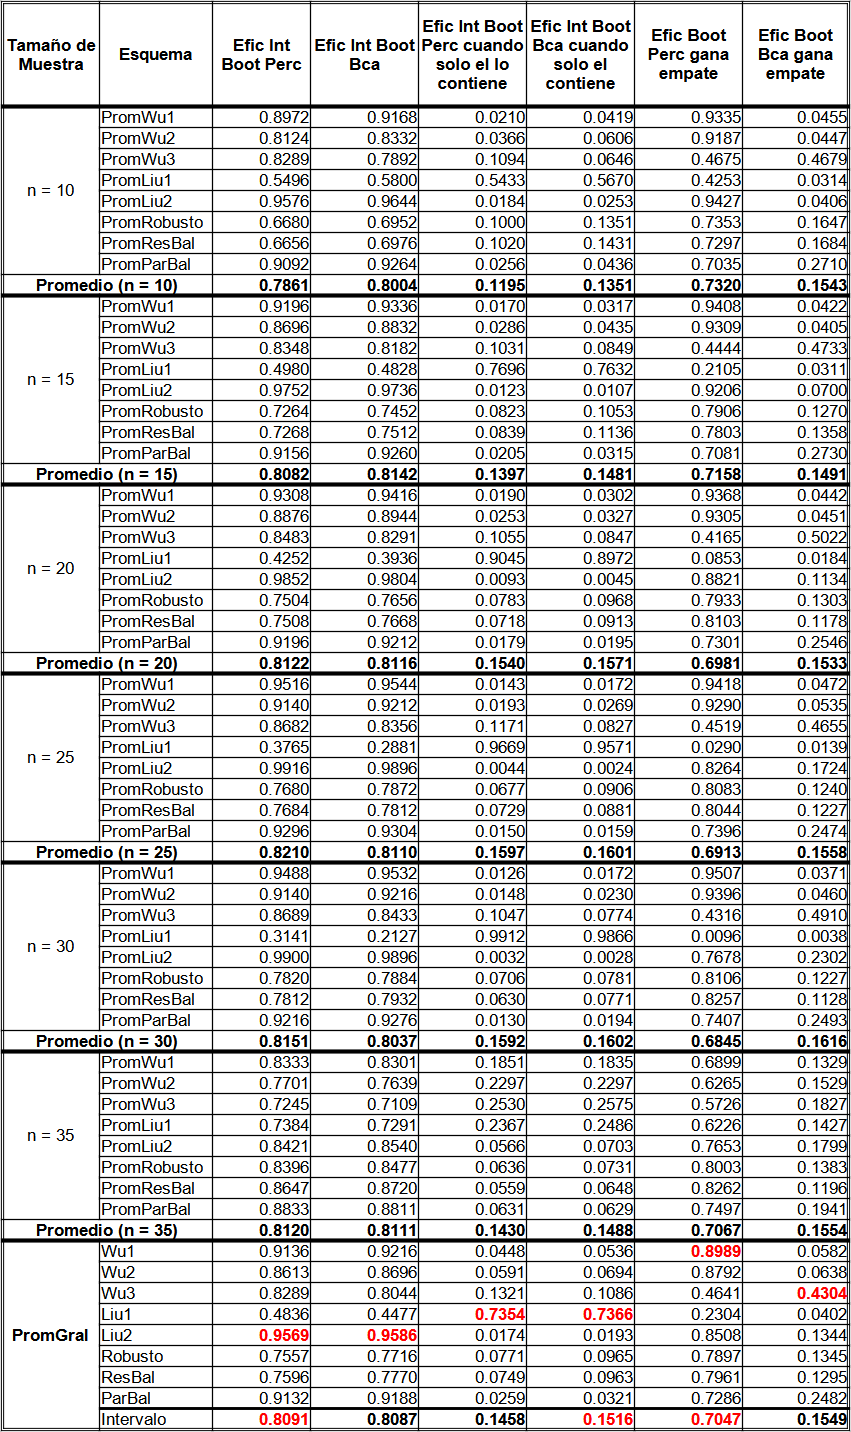
\includegraphics[width=0.55\linewidth]{img/EP_NVC_Efic_Boots.png} 
	\caption{Eficiencia promedio de los intervalos Bootstrap por tamaño de muestra y esquema de remuestreos para el caso EP-NVC.} 
	\label{fig:EficPromIntBootsTamMuestEsqRemuEP-NVC}
\end{figure}

\FloatBarrier

\subsubsection{Eficiencia de los esquemas para el caso EP-NVC}
Con base en el promedio de eficiencia por tamaño de muestra (Figura \ref{fig:EficPromEsqTamMuesEsqRemuEP-NVC}) y un nivel de confianza mayor o igual a 0.95: con tamaño de muestra 10 ningún esquema cumplió la condición, sin embargo con Liu2 se obtuvo 0.94, y con los tamaños de muestra 15, 20, 25, 30 y 35 el mejor fue es el esquema Lui2.\\


Sin considerar el tamaño de la muestra, para el caso EP-NVC el mejor promedio general (Figura \ref{fig:EficPromEsqTamMuesEsqRemuEP-NVC}) en eficiencia de esquema es Liu2 (0.9737).


\begin{figure}[H] 
	\centering 
	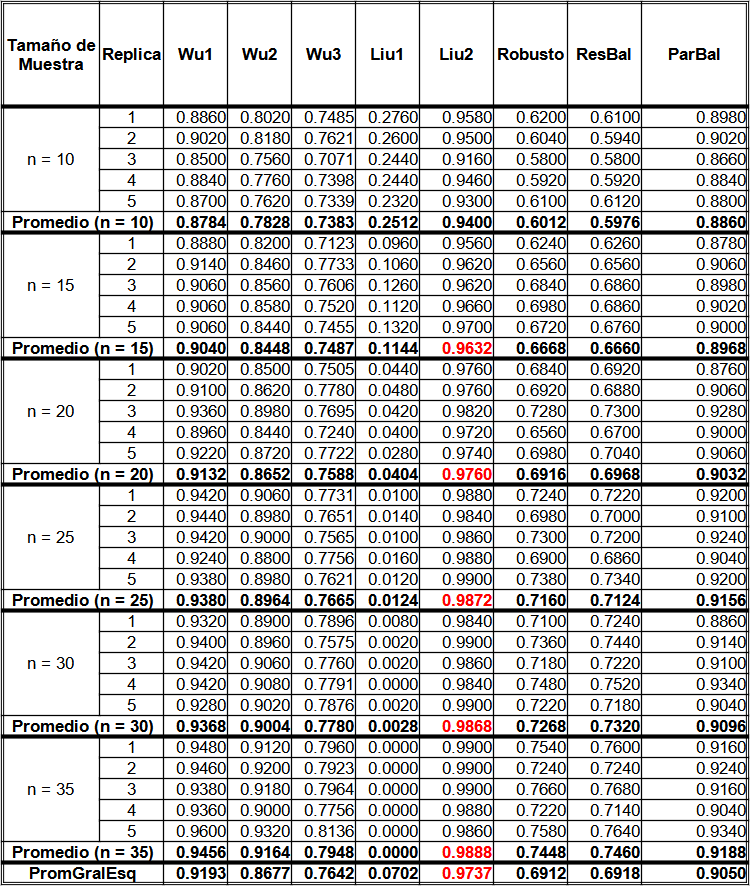
\includegraphics[width=0.70\linewidth]{img/EP_NVC_Efic_Esq.png} 
	\caption{Eficiencia promedio de los esquemas por tamaño de muestra y esquema de remuestreos para el caso EP-NVC.} 
	\label{fig:EficPromEsqTamMuesEsqRemuEP-NVC}
\end{figure}

\FloatBarrier

%%%%%%%%%%%%%%%%%%%%%%%%%%%%%%%%%%%%%%%%%%%
\subsubsection{Eficiencia de los intervalos Bootstrap para el caso EP-NNVC}
Con base en el promedio general (Figura \ref{fig:EficPromIntBootsTamMuestEsqRemuEP-NNVC}) para: Eficiencia del ICB Percentil (Efic Int Boot Perc) y Eficiencia en ICB BCa (Efic Int Boot Bca) el mejor esquema resulto Liu2, 0.9893 y 0.9870 respectivamente;
Eficiencia del ICB Percentil cuando solo el lo contiene a la $R^{2}$ y Eficiencia del ICB BCa cuando solo el contiene a la $R^{2}$ el mejor esquema es Liu1, 0.6381 y 0.6549 respectivamente; 
la Eficiencia de ICB Percentil cuando gana en el empate a ICB BCa (Efic Boot Perc gana empate), el mejor esquema es Wu2 $(0.9026)$ y la Eficiencia ICB BCa cuando gana el empate al ICB Percentil (Efic Boot Bca gana empate), el mejor esquema es Wu3 $(0.8147)$.\\


%Poner el contexto
Sin considerar el tamaño de la muestra, para el caso EP-NNVC los ICB mejores en promedio general  (Figura \ref{fig:EficPromIntBootsTamMuestEsqRemuEP-NNVC}) son: Eficiencia del ICB BCa (Efic Int Boot Bca) con $0.8653$ ante la Eficiencia en ICB Percentil (Efic Int Boot Perc); la Eficiencia del ICB BCa cuando solo el contiene a la $R^{2}$ $(0.1117)$ y la Eficiencia de ICB Percentil cuando gana en el empate al ICB BCa (Efic Boot Perc gana empate) con $0.6697$.



\begin{figure}[ht] 
	\centering 
	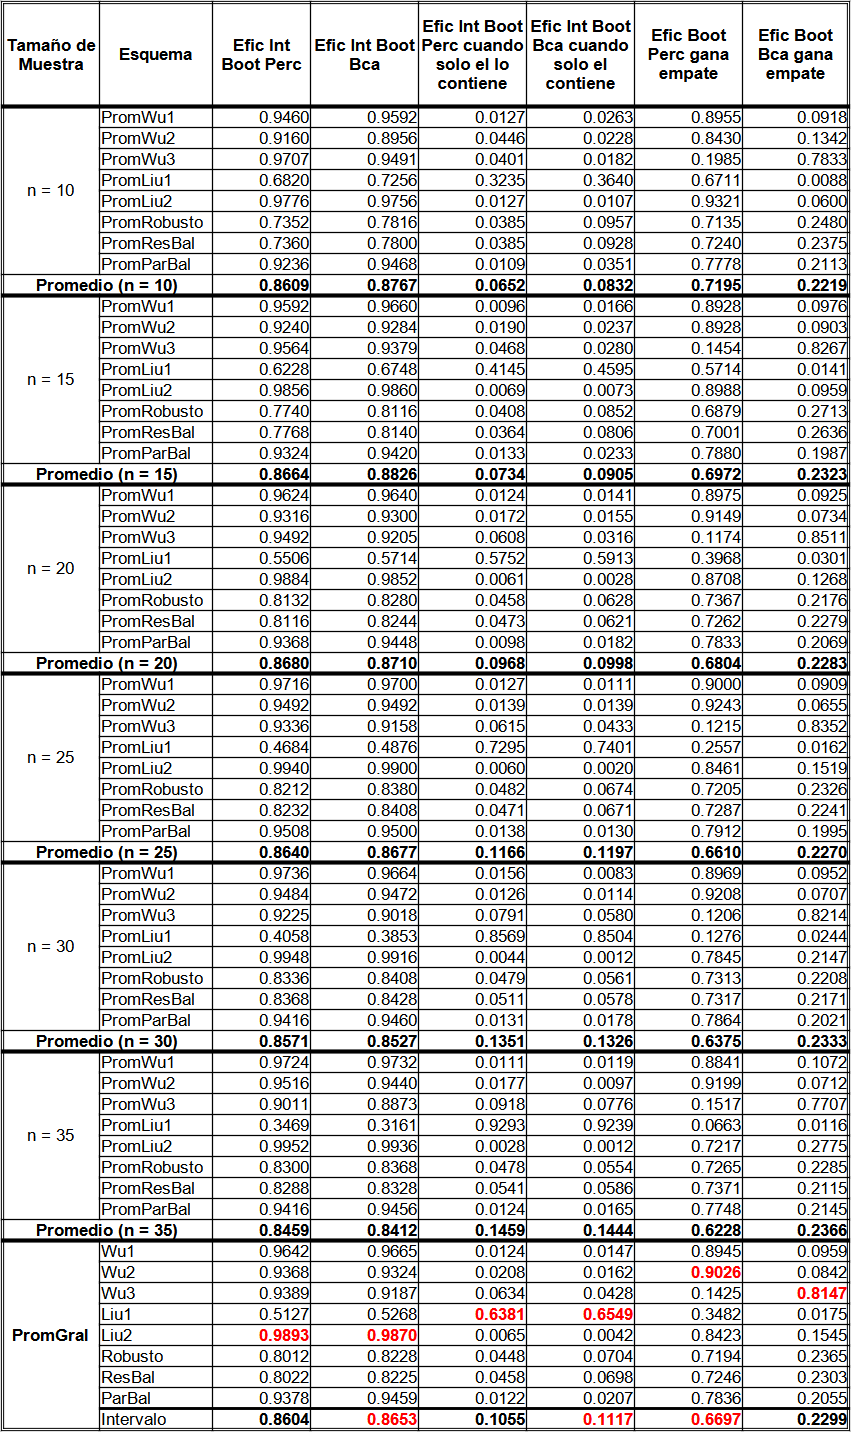
\includegraphics[width=0.55\linewidth]{img/EP_NNVC_Efic_Boots.png} 
	\caption{Eficiencia promedio de los intervalos Bootstrap por tamaño de muestra y esquema de remuestreos para el caso EP-NNVC.} 
	\label{fig:EficPromIntBootsTamMuestEsqRemuEP-NNVC}
\end{figure}
\FloatBarrier


\subsubsection{Eficiencia de los esquemas para el caso EP-NNVC}
Con base en el promedio de eficiencia por tamaño de muestra (Figura \ref{fig:EficPromEsqTamMuesEsqRemuEP-NNVC}) y un nivel de confianza mayor o igual a 0.95: con tamaño de muestra 10 el mejor fue el esquema Liu2 (0.9651), seguido por Wu1 (0.9340) y con los tamaños de muestra 15, 20, 25, 30 y 35 los mejores esquemas son Liu2 y Wu1.\\

Sin considerar el tamaño de la muestra, para el caso EP-NNVC los mejores promedio generales (Figura \ref{fig:EficPromEsqTamMuesEsqRemuEP-NNVC}) en eficiencia son los esquema Liu2 y Wu1.


\begin{figure}[ht] 
	\centering 
	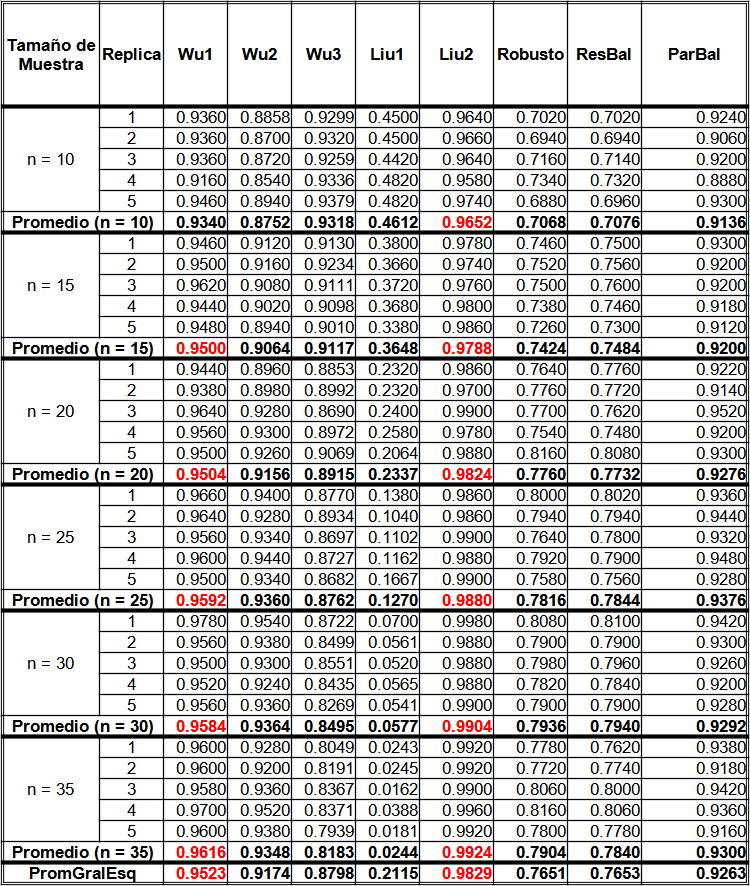
\includegraphics[width=0.70\linewidth]{img/EP_NNVC_Efic_Esq.png} 
	\caption{Eficiencia promedio de los esquemas por tamaño de muestra y esquema de remuestreos para el caso EP-NNVC.} 
	\label{fig:EficPromEsqTamMuesEsqRemuEP-NNVC}
\end{figure}
\FloatBarrier


%%%%%%%%%%%%%%%%%%%%%%%%%%%%%%%%%%%%%%%%%%%%%%%%

\subsubsection{Eficiencia de los intervalos Bootstrap para el caso EP-NVD}
Con base en el promedio general (Figura \ref{fig:EficPromIntBootsTamMuestEsqRemuEP-NVD}) para: Eficiencia del ICB Percentil (Efic Int Boot Perc) y Eficiencia en ICB BCa (Efic Int Boot Bca) el mejor esquema resulto Liu2, 0.9775 y 0.9760 respectivamente; Eficiencia del ICB Percentil cuando solo el lo contiene a la $R^{2}$ y Eficiencia del ICB BCa cuando solo el contiene a la $R^{2}$ el mejor esquema es Liu1, 0.5042 y 0.4677 respectivamente; 
la Eficiencia de ICB Percentil cuando gana en el empate a ICB BCa (Efic Boot Perc gana empate), el mejor esquema es Pareado Balanceado (ParBal) con 0.8230 y la Eficiencia ICB BCa cuando gana el empate al ICB Percentil, el mejor esquema es Wu3 $(0.5159)$.\\


Sin considerar el tamaño de la muestra, para el caso EP-NVD los ICB mejores en promedio general (Figura \ref{fig:EficPromIntBootsTamMuestEsqRemuEP-NVD}) son: Eficiencia del ICB BCa (Efic Int Boot Bca) con $0.8299$ ante la Eficiencia en ICB Percentil (Efic Int Boot Perc); la Eficiencia del ICB Percentil cuando solo el contiene a la $R^{2}$ $(0.1049)$ y la Eficiencia de ICB BCa cuando gana en el empate al ICB Percentil (Efic Boot Bca gana empate) con $0.2942$.


\begin{figure}[ht] 
	\centering 
	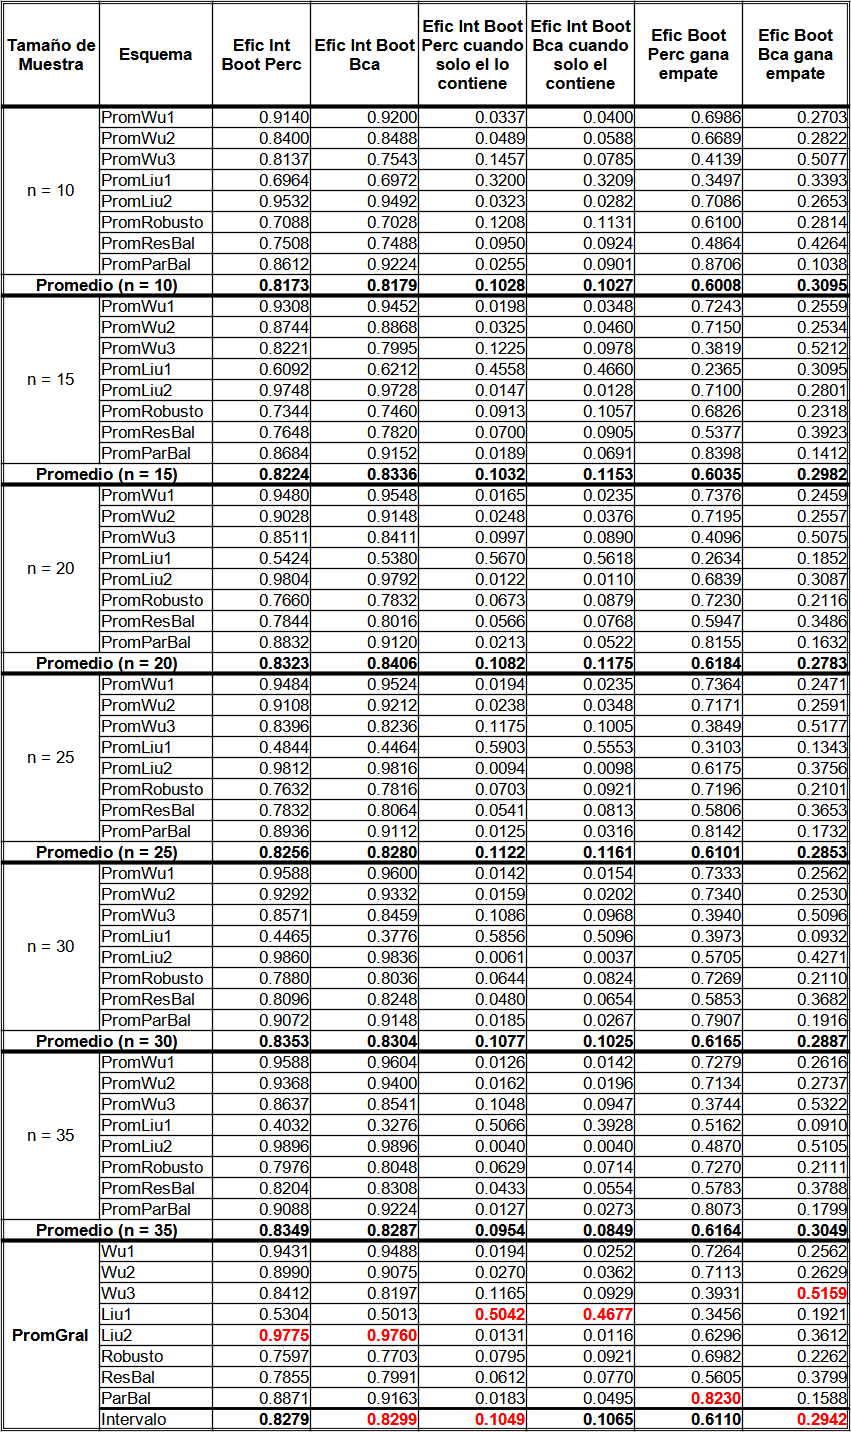
\includegraphics[width=0.55\linewidth]{img/EP_NVD_Efic_Boots.png} 
	\caption{Eficiencia promedio de los intervalos Bootstrap por tamaño de muestra y esquema de remuestreos para el caso EP-NVD.} 
	\label{fig:EficPromIntBootsTamMuestEsqRemuEP-NVD}
\end{figure}
\FloatBarrier

\subsubsection{Eficiencia de los esquemas para el caso EP-NVD}
Con base en el promedio de eficiencia por tamaño de muestra (Figura \ref{fig:EficPromEsqTamMuesEsqRemuEP-NVD}) y un nivel de confianza mayor o igual a 0.95: con tamaño de muestra 10 ningún esquema cumplió la condición, sin embargo con Liu2 se obtuvo 0.9224 y con los tamaños de muestra 15, 20, 25, 30 y 35 el mejor fue el esquema Lui2.\\

Sin considerar el tamaño de la muestra, para el caso EP-NVD el mejor promedio general (Figura \ref{fig:EficPromEsqTamMuesEsqRemuEP-NVD}) en eficiencia de esquema es Liu2 (0.9648).


\begin{figure}[ht] 
	\centering 
	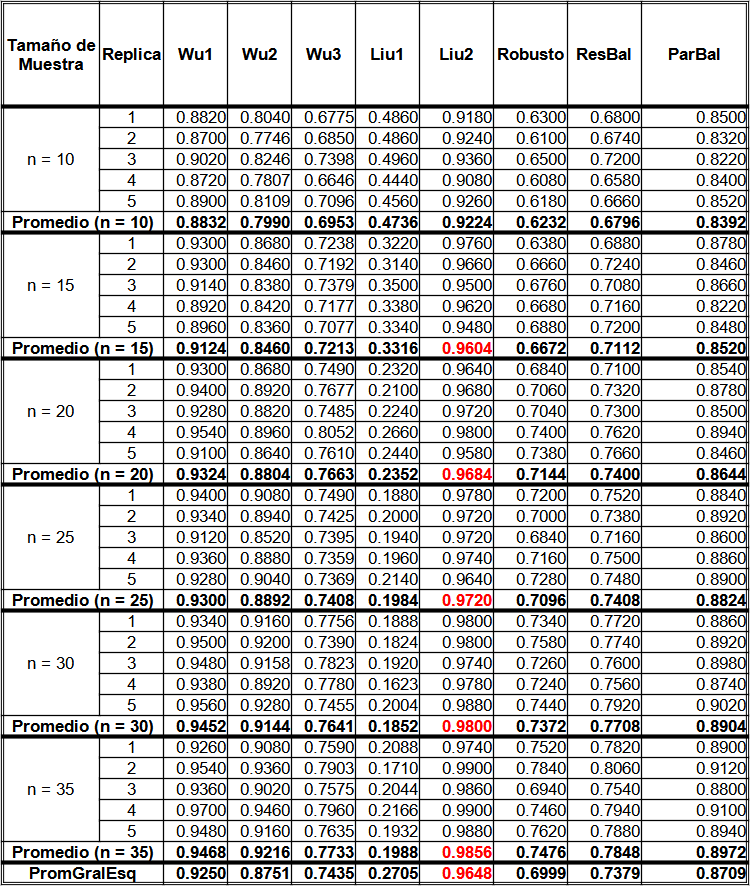
\includegraphics[width=0.70\linewidth]{img/EP_NVD_Efic_Esq.png} 
	\caption{Eficiencia promedio de los esquemas por tamaño de muestra y esquema de remuestreos para el caso EP-NVD.} 
	\label{fig:EficPromEsqTamMuesEsqRemuEP-NVD}
\end{figure}
\FloatBarrier


%%%%%%%%%%%%%%%%%%%%%%%%%%%%%%%%%

\subsubsection{Eficiencia de los intervalos Bootstrap para el caso EP-NNVD}
Con base en el promedio general (Figura \ref{fig:EficPromIntBootsTamMuestEsqRemuEP-NNVD}) para: Eficiencia del ICB Percentil (Efic Int Boot Perc) el mejor esquema resulto Liu2 (0.9171); 
Eficiencia en ICB BCa (Efic Int Boot Bca) el mejor esquema resulto Pareado Balanceado (ParBal) con 0.9162;
 Eficiencia del ICB Percentil cuando solo el lo contiene a la $R^{2}$ y Eficiencia del ICB BCa cuando solo el contiene a la $R^{2}$ el mejor esquema resulto Wu3, 0.3156 y 0.2458 respectivamente;
 la Eficiencia de ICB Percentil cuando gana en el empate a ICB BCa (Efic Boot Perc gana empate), el mejor esquema es ParBal (0.7930) y la Eficiencia ICB BCa cuando gana el empate al ICB Percentil (Efic Boot Bca gana empate), el mejor esquema es de Residuales Balanceados (ResBal) con 0.8630.\\


Sin considerar el tamaño de la muestra, para el caso EP-NNVD los ICB mejores en promedio general  (Figura \ref{fig:EficPromIntBootsTamMuestEsqRemuEP-NNVD}) son: Eficiencia del ICB Percentil (Efic Int Boot Perc) con $0.8186$ ante la Eficiencia en ICB BCa (Efic Int Boot Bca); la Eficiencia del ICB Percentil cuando solo el contiene a la $R^{2}$ $(0.1119)$ y la Eficiencia de ICB BCa cuando gana en el empate al ICB Perc (Efic Boot Bca gana empate) con $0.6286$.


\begin{figure}[ht] 
	\centering 
	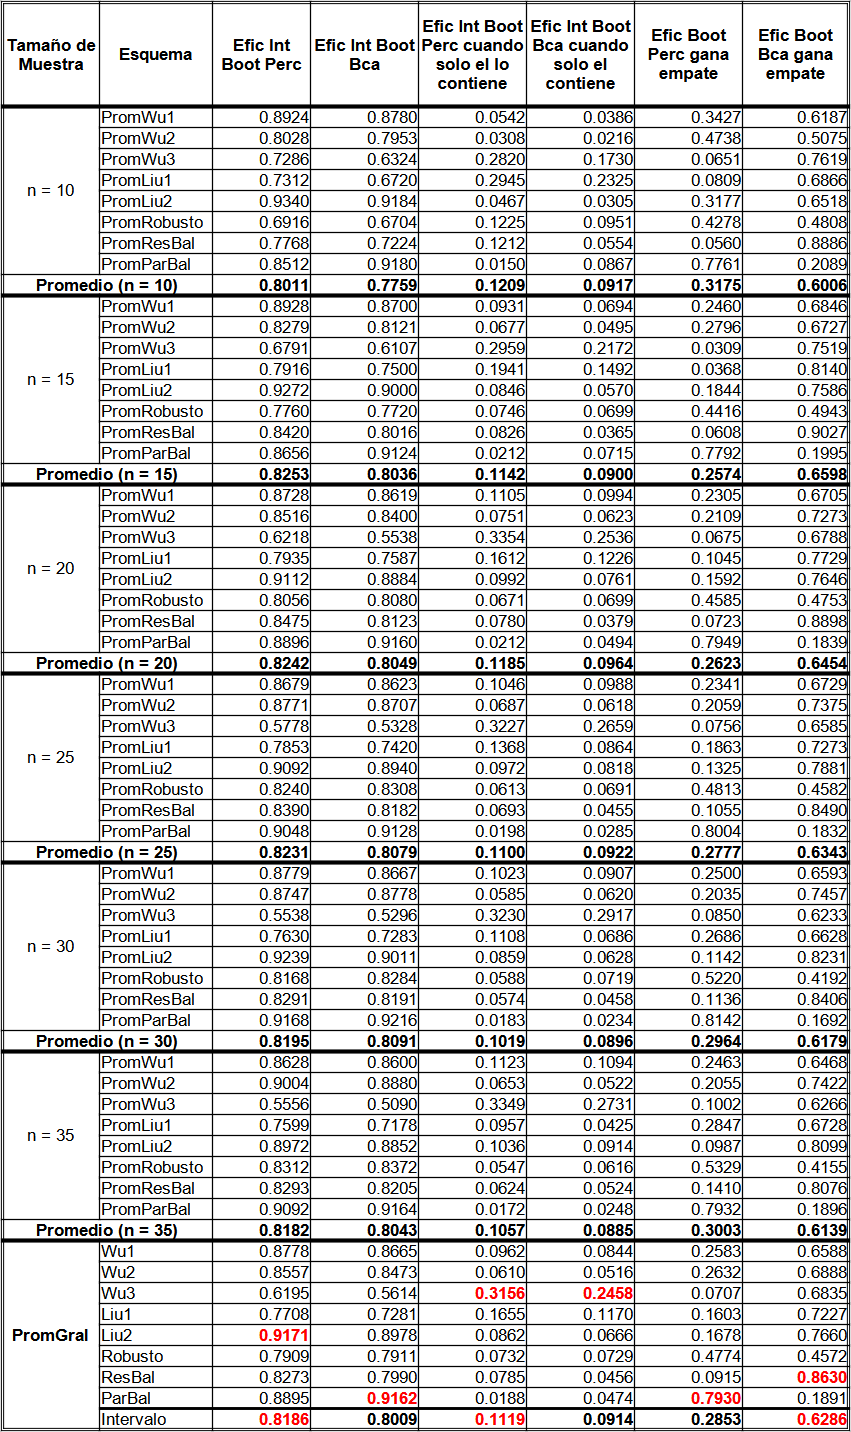
\includegraphics[width=0.55\linewidth]{img/EP_NNVD_Efic_Boots.png} 
	\caption{Eficiencia promedio de los intervalos Bootstrap por tamaño de muestra y esquema de remuestreos para el caso EP-NNVD.} 
	\label{fig:EficPromIntBootsTamMuestEsqRemuEP-NNVD}
\end{figure}
\FloatBarrier

\subsubsection{Eficiencia de los esquemas para el caso EP-NNVD}
Con base en el promedio de eficiencia por tamaño de muestra (Figura \ref{fig:EficPromEsqTamMuesEsqRemuEP-NNVD}) y un nivel de confianza mayor o igual de 0.90: solo con el tamaño de muestra 30 se cumple la condición bajo el esquema Pareado Balanceado (ParBal) con 0.9. Ahora sin considerar el criterio anterior, el mejor esquema para: n=10 es Liu2 (0.8904) y Wu1(0.8440), n=15 es Liu2 (0.8488) y ParBal (0.8472), n=20 es ParBal (0.8708) y Liu2 (0.8207), n=25 es ParBal (0.8868) y Liu2 (0.8207), n=30 es ParBal (0.9) y Liu2 (0.8447) y en n=35 es ParBal (0.8936) y Wu2 (0.8415). \\


Sin considerar el tamaño de la muestra, para el caso EP-NNVD los mejores promedios generales (Figura \ref{fig:EficPromEsqTamMuesEsqRemuEP-NNVD}) en eficiencia de esquema son ParBal (0.8728) y Liu2 (0.8383).


\begin{figure}[ht] 
	\centering 
	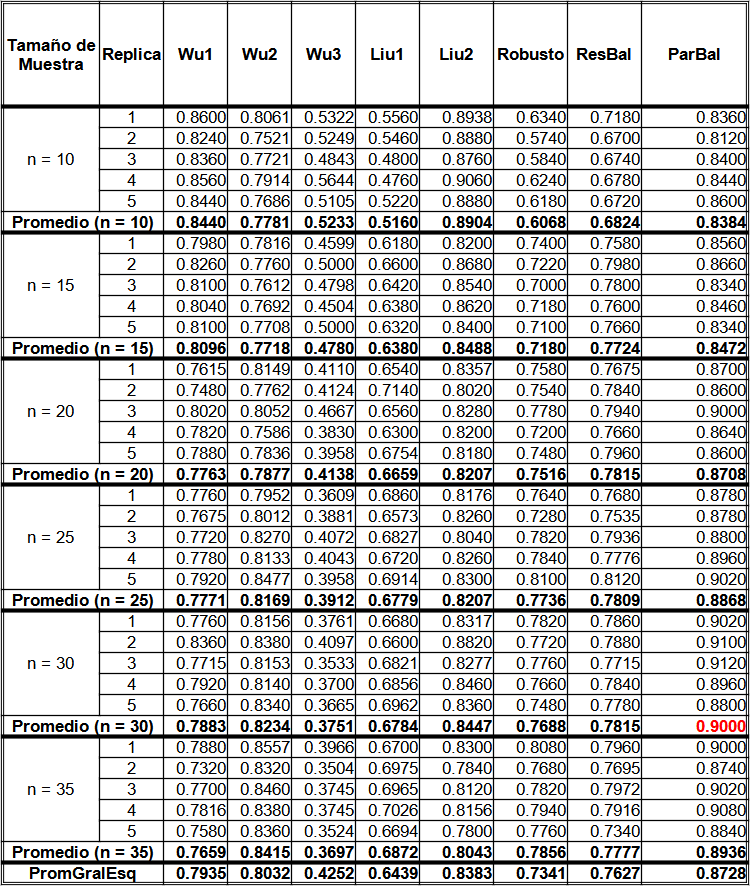
\includegraphics[width=0.70\linewidth]{img/EP_NNVD_Efic_Esq.png} 
	\caption{Eficiencia promedio de los esquemas por tamaño de muestra y esquema de remuestreos para el caso EP-NNVD.} 
	\label{fig:EficPromEsqTamMuesEsqRemuEP-NNVD}
\end{figure}
\FloatBarrier

%%Tipo de intervalo y esquema para evaluar la precision. 8 recomendaciones

%%%%%%%%%%%%%%%%%%%

\subsubsection{Promedio de supuestos para el caso EP}
Dados los modelos de tipo EP para los casos: NVC, NNVC y NVD, con base en los promedios generales (Figura \ref{fig:PromSupuUtiliEP}), por encima del 95\% se recomienda el uso del esquema Liu 2 con el intervalo Percentil; y por encima del 90\% para NNVD de igual forma el esquema Liu 2, pero con el intervalo BCa, para la evaluación de precisión.


\begin{figure}[ht] 
	\centering 
	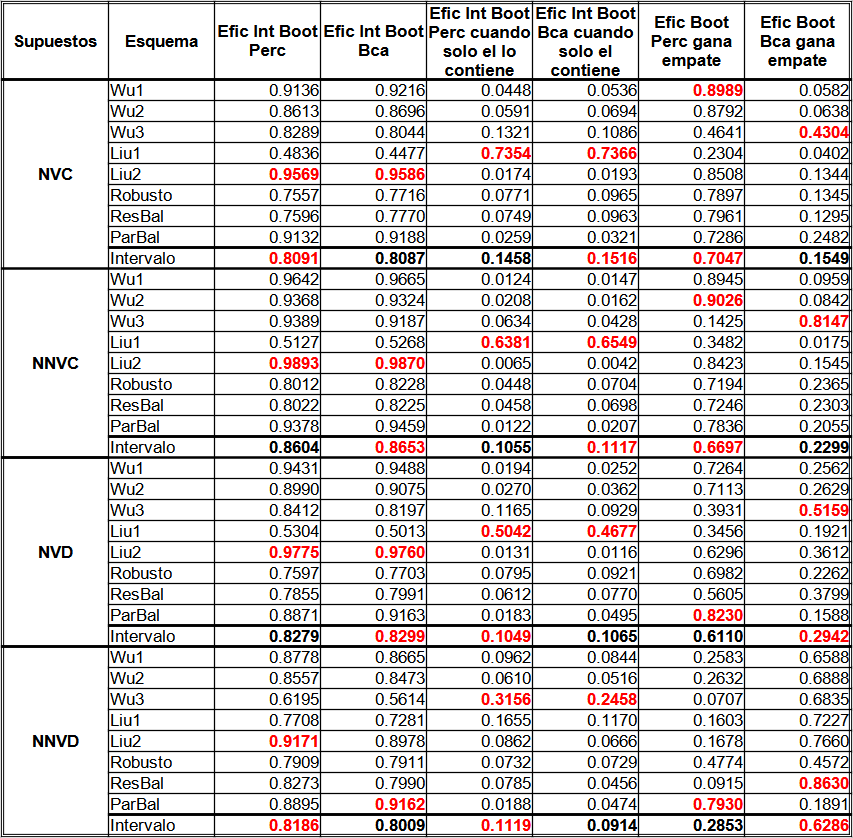
\includegraphics[width=0.80\linewidth]{img/EP_Prom_Supuestos.png} 
	\caption{Promedio de supuestos utilizados para el caso EP.} 
	\label{fig:PromSupuUtiliEP}
\end{figure}
\FloatBarrier



%%%%%%%%%%%%%%%%%%%%%%%%%%%%%%%%%%%%%%%%%%%%%%%%%%%%%%%%%%%%%%%%%%%%%%%%%%%%%%%%%%%%%%%%%%%

%%%%%%%%%%%%%%%%%%%%%%%%%%%%%%Empieza EI

\subsubsection{Eficiencia de los intervalos Bootstrap para el caso EI-NVC}
Con base en el promedio general (Figura \ref{fig:EficPromIntBootsTamMuestEsqRemuEI-NVC}) para: Eficiencia del ICB Percentil (Efic Int Boot Perc) y Eficiencia en ICB BCa (Efic Int Boot Bca) el mejor esquema resulto Liu2, 0.9627 y 0.9052 respectivamente;
 Eficiencia del ICB Percentil cuando solo el lo contiene a la $R^{2}$ y Eficiencia del ICB BCa cuando solo el contiene a la $R^{2}$ el mejor esquema resulto Liu1, 0.5864 y 0.5751 respectivamente; 
 la Eficiencia de ICB Percentil cuando gana en el empate a ICB BCa (Efic Boot Perc gana empate), el mejor esquema es Wu3 (0.3019) y la Eficiencia ICB BCa cuando gana el empate al ICB Percentil (Efic Boot Bca gana empate), el mejor esquema es Wu2 (0.8626).\\


Sin considerar el tamaño de la muestra, para el caso EI-NVC los ICB mejores en promedio general (Figura \ref{fig:EficPromIntBootsTamMuestEsqRemuEI-NVC}) son: Eficiencia del ICB Percentil (Efic Int Boot Perc) con $0.8745$ ante la Eficiencia en ICB BCa (Efic Int Boot Bca); la Eficiencia del ICB Percentil cuando solo el contiene a la $R^{2}$ $(0.1413)$ y la Eficiencia de ICB BCa cuando gana en el empate al ICB Perc (Efic Boot Bca gana empate) con $0.7469$.


\subsubsection{Eficiencia de los esquemas para el caso EI-NVC}
Con base en el promedio de eficiencia por tamaño de muestra (Figura \ref{fig:EficPromEsqTamMuesEsqRemuEI-NVC}) y un nivel de confianza mayor o igual a 0.90: con tamaño de muestra 10 y 15 ningún esquema cumplió la condición, sin embargo con ambos el mejor esquema es Liu2, con 0.8227 y 0.8639 respectivamente; con los tamaños de muestra 20, 25, 30 el mejor fue el esquema Lui2 y con el tamaño de muestra 35 los mejores esquemas fueron Wu1, Wu2, Liu2 y Pareado Balanceado (ParBal).\\

Sin considerar el tamaño de la muestra, para el caso EI-NVC el mejor promedio general (Figura \ref{fig:EficPromEsqTamMuesEsqRemuEI-NVC}) en eficiencia de esquema es Liu2 (0.8938).




%%%%%%%%%%%%%%%%%%%%%%%%%%%%%%%%%%%%%%%

\subsubsection{Eficiencia de los intervalos Bootstrap para el caso EI-NNVC}
Con base en el promedio general (Figura \ref{fig:EficPromIntBootsTamMuestEsqRemuEI-NNVC}) para: Eficiencia del ICB Percentil (Efic Int Boot Perc) y Eficiencia en ICB BCa (Efic Int Boot Bca) el mejor esquema resulto Liu2, 0.9603 y 0.9005 respectivamente;
 Eficiencia del ICB Percentil cuando solo el lo contiene a la $R^{2}$ y Eficiencia del ICB BCa cuando solo el contiene a la $R^{2}$ el mejor esquema resulto Liu1, 0.5224 y 0.5304 respectivamente; la Eficiencia de ICB Percentil cuando gana en el empate a ICB BCa (Efic Boot Perc gana empate), el mejor esquema es Wu3 (0.6169) y la Eficiencia ICB BCa cuando gana el empate al ICB Percentil (Efic Boot Bca gana empate), el mejor esquema es Pareado Balanceado (ParBal) con 0.7493.\\

Sin considerar el tamaño de la muestra, para el caso EI-NNVC los ICB mejores en promedio general (Figura \ref{fig:EficPromIntBootsTamMuestEsqRemuEI-NNVC}) son: Eficiencia del ICB Percentil (Efic Int Boot Perc) con $0.8833$ ante la Eficiencia en ICB BCa (Efic Int Boot Bca); la Eficiencia del ICB Percentil cuando solo el contiene a la $R^{2}$ $(0.1467)$ y la Eficiencia de ICB BCa cuando gana en el empate al ICB Perc (Efic Boot Bca gana empate) con $0.6252$.




\subsubsection{Eficiencia de los esquemas para el caso EI-NNVC}
Con base en el promedio de eficiencia por tamaño de muestra (Figura \ref{fig:EficPromEsqTamMuesEsqRemuEI-NNVC})  y un nivel de confianza mayor o igual a 0.90: con los tamaños de muestra 10, 15 y 20 ningún esquema cumplió la condición, sin embargo, al no considerar el criterio anterior, el mejor esquema para: n=10 es Wu3 (0.8252) y Liu2 (0.8215), n=15 es Liu2 (0.8515) y Pareado Balanceado (ParBar) con 0.8352 y n=20 es Liu2 (0.8800) y Wu1 (0.8532). Con el tamaño de muestra 25 el mejor esquema es Liu2 (0.9116) seguido por ParBal (0.8932), con tamaño de muestra 30 el mejor esquema es Liu2 (0.9140) seguido por ParBal (0.8956) y con el tamaño de muestra 35 los mejores esquemas son Liu2 y ParBal, con 0.9288 y 0.904 respectivamente.\\

Sin considerar el tamaño de la muestra, para el caso EI-NNVC los mejores promedios generales (Figura \ref{fig:EficPromEsqTamMuesEsqRemuEI-NNVC})  en eficiencia de esquema son Liu2 (0.8848) y ParBal (0.8671).




%%%%%%%%%%%%%%%%%%%%%%%%%%%%%%%
\subsubsection{Eficiencia de los intervalos Bootstrap para el caso EI-NVD}
Con base en el promedio general  (Figura \ref{fig:EficPromIntBootsTamMuestEsqRemuEI-NVD}) para: Eficiencia del ICB Percentil (Efic Int Boot Perc) el mejor esquema resulto Liu2 (0.9837), Eficiencia en ICB BCa (Efic Int Boot Bca) el mejor esquema resulto Pareado Balanceado(ParBal) con 0.8915; Eficiencia del ICB Percentil cuando solo el lo contiene a la $R^{2}$ y Eficiencia del ICB Bca cuando solo el contiene a la $R^{2}$ el mejor esquema resulto Liu1, 0.3799 y 0.3885 respectivamente; la Eficiencia de ICB Percentil cuando gana en el empate a ICB BCa (Efic Boot Perc gana empate), el mejor esquema es Residuales Balanceados(ResBal) con 0.3364 y la Eficiencia ICB BCa cuando gana el empate al ICB Percentil (Efic Boot Bca gana empate), el mejor esquema es Wu2 (0.7012).\\


Sin considerar el tamaño de la muestra, para el caso EI-NVD los ICB mejores en promedio general  (Figura \ref{fig:EficPromIntBootsTamMuestEsqRemuEI-NVD}) son: Eficiencia del ICB Percentil (Efic Int Boot Perc) con $0.9030$ ante la Eficiencia en ICB BCa (Efic Int Boot Bca); la Eficiencia del ICB Percentil cuando solo el contiene a la $R^{2}$ $(0.1402)$ y la Eficiencia de ICB BCa cuando gana en el empate al ICB Perc (Efic Boot Bca gana empate) con $0.6501$.



\subsubsection{Eficiencia de los esquemas para el caso EI-NVD}
Con base en el promedio de eficiencia por tamaño de muestra (Figura \ref{fig:EficPromEsqTamMuesEsqRemuEI-NVD}) y un nivel de confianza mayor o igual a 0.90: con tamaño de muestra 10, 15 y 20 ningún esquema cumplió la condición,
sin embargo, al no considerar el criterio anterior, el mejor esquema para: n=10 es Pareado Balanceado (ParBal) con 0.8110, Liu2 (0.7977), Wu1 (0.7829) y Wu2 (0.7637); n=15 es Liu2 (0.8463), ParBal (0.8419), Wu1 (0.8415) y Wu2 (0.8255), y n=20 Liu2 (0.8708), ParBal (0.8612), Wu1 (0.8591) y Wu2 (0.7637). Con el tamaño de muestra 25 el mejor esquema es Liu2 (0.9035) seguido por ParBal (0.8932), Wu1 (0.8892) y Wu2 (0.881); con tamaño de muestra 30 los mejores esquemas son Liu2 (0.9236),  Wu1 (0.9160), ParBal (0.9152) y Wu2 (0.9088), y con el tamaño de muestra 35 los mejores esquemas son Liu2 (0.9348),  Wu1 (0.9256), ParBal (0.922) y Wu2 (0.92).\\

Sin considerar el tamaño de la muestra, para el caso EI-NVD el mejor promedio general (Figura \ref{fig:EficPromEsqTamMuesEsqRemuEI-NVD}) en eficiencia de esquema son Liu2 (0.8794), ParBal (0.8741), Wu1 (0.8690) y Wu2 (0.8583).




%%%%%%%%%%%%%%%%%%%%%%%%%%%%%%%%
\subsubsection{Eficiencia de los intervalos Bootstrap para el caso EI-NNVD}
Con base en el promedio general (Figura \ref{fig:EficPromIntBootsTamMuestEsqRemuEI-NNVD}) para: Eficiencia del ICB Percentil (Efic Int Boot Perc) el mejor esquema resulto Liu2 (0.9554), Eficiencia en ICB BCa (Efic Int Boot Bca) el mejor esquema resulto Pareado Balanceado (ParBal) con 0.8882; Eficiencia del ICB Percentil cuando solo el lo contiene a la $R^{2}$ el mejor esquema resulto Wu3 (0.2807), Eficiencia del ICB BCa cuando solo el contiene a la $R^{2}$ el mejor esquema resulto Liu1 (0.1632); la Eficiencia de ICB Percentil cuando gana en el empate a ICB BCa (Efic Boot Perc gana empate), el mejor esquema es Residuales Balanceados(ResBal) con 0.5197 y la Eficiencia ICB BCa cuando gana el empate al ICB Percentil (Efic Boot Bca gana empate), el mejor esquema es ParBal (0.5074).\\

Sin considerar el tamaño de la muestra, para el caso EI-NNVD los ICB mejores en promedio general (Figura \ref{fig:EficPromIntBootsTamMuestEsqRemuEI-NNVD}) son: Eficiencia del ICB Percentil (Efic Int Boot Perc) con $0.9035$ ante la Eficiencia en ICB BCa (Efic Int Boot Bca); la Eficiencia del ICB Percentil cuando solo el contiene a la $R^{2}$ $(0.1940)$ y la Eficiencia de ICB BCa cuando gana en el empate al ICB Perc (Efic Boot Bca gana empate) con $0.5074$.



\subsubsection{Eficiencia de los esquemas para el caso EI-NNVD}
Con base en el promedio de eficiencia por tamaño de muestra (Figura \ref{fig:EficPromEsqTamMuesEsqRemuEI-NNVD}) y un nivel de confianza mayor o igual a 0.90: con tamaño de muestra 10, 15, 20 y 25 ningún esquema cumplió la condición, sin embargo, al no considerar el criterio anterior, el mejor esquema para: n=10 es Pareado Balanceado (ParBal) con 0.7936; n=15 es (ParBal) con 0.8387;  n=20 es ParBal (0.8680) y  n=25 es ParBal (0.8932). Con los tamaños de muestra 30 y 35 el mejor esquema es ParBal, 0.91 y 0.9240 respectivamente.\\

Sin considerar el tamaño de la muestra, para el caso EI-NNVD el mejor promedio general (Figura \ref{fig:EficPromEsqTamMuesEsqRemuEI-NNVD}) en eficiencia de esquema es ParBal (0.8713).




%%%%%%%%%%%%%%%%%%%
\subsubsection{Promedio de supuestos para el caso EI}
Dados los modelos de tipo EI para los casos: NVC, NNVC, NVD y NNVD con base en los promedios generales(Figura \ref{fig:PromSupuUtiliEI}), por encima del 95\% se recomienda el uso del esquema Liu 2 con el intervalo BCa, para la evaluación de precisión.






%%%%%%%%%%%%%%%%%%%%%%%%%%%%%%%%%%%%%%%%%%%%%%%%%%%%%%%%%%%%%%%%%%%%%%%%
%%%%%%%%%%%%%%%%%%%%%Estadistica fuerte

\subsubsection{Comparación de la eficiencia del ICB Percentil cuando se tiene NVC (NVC-EficIB1)}

Cuando se tiene NVC y se utilizó el ICB-perc para evaluar la precisión, se obtuvo interacción triple significativa ($TipoMod \times TM \times Esq: F=11.97, P<0.0001$; Tabla \ref{fig:ANOVA_Efic_ICB_Perc_NVC} del Anexo B ). Con base en una eficiencia promedio de al menos 95\%, el mejor esquema resultó Liu2 sin importar el tamaño de muestra y tipo de modelo (Tabla \ref{fig:CompEfic_PromICB_Perc_NVC}).\\


\begin{figure}[ht] 
	\centering 
	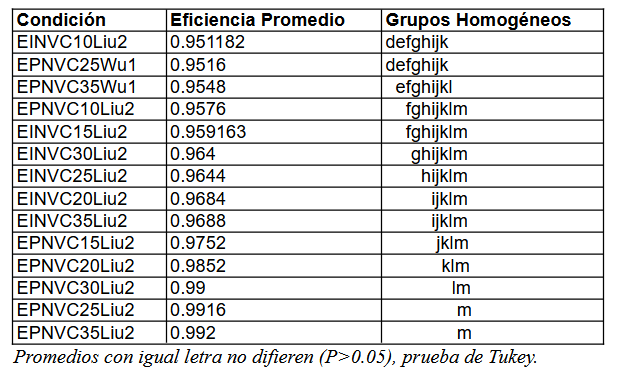
\includegraphics[width=0.76\linewidth]{img/CompEfic_PromICB_Perc_NVC.png} 
	\caption{Comparación de eficiencias promedio del ICB Percentil cuando se tiene NVC.} 
	\label{fig:CompEfic_PromICB_Perc_NVC}
\end{figure}
\FloatBarrier



\subsubsection{Comparación de la eficiencia del ICB BCa cuando se tiene NVC (NVC-EficIB2)}

Cuando se tiene NVC y se utilizó el ICB-BCa para evaluar la precisión, se obtuvo interacción triple significativa ($TipoMod*TM*Esq: F=3.60, P<0.0001;$ Tabla \ref{fig:ANOVA_Efic_ICB_BCa_NVC} del Anexo B). Con base en una eficiencia promedio de al menos 95\%, el mejor esquema resultó Liu2 sin importar el TM, sin embargo, sólo identifica al tipo de modelo EP a priori simulado (Tabla \ref{fig:CompEfic_PromICB_BCa_NVC}).\\



\begin{figure}[ht] 
	\centering 
	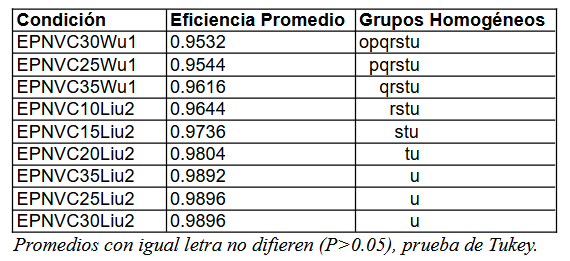
\includegraphics[width=0.76\linewidth]{img/CompEfic_PromICB_BCa_NVC.png} 
	\caption{Comparación de eficiencias promedio del ICB BCa cuando se tiene NVC.} 
	\label{fig:CompEfic_PromICB_BCa_NVC}
\end{figure}
\FloatBarrier



%%%%%%%%%%%%%%%%%%%%%%%%%%%5

\subsubsection{Comparación de la eficiencia del ICB percentil cuando se tiene NNVC (NNVC-EficIB1)}

Cuando se tiene NNVC y se utilizó el ICB-perc para evaluar la precisión, se obtuvo interacción triple significativa ($TipoMod*TM*Esq: F=17.86, P<0.0001$;Tabla \ref{fig:ANOVA_Efic_ICB_Perc_NNVC} del Anexo B). Con base en una eficiencia promedio de al menos 95\%, el mejor esquema resultó Liu2 sin importar el tamaño de muestra y tipo de modelo; con excepción del caso EINNVC10Liu2, sin embargo, su eficiencia promedio es 94.52\% (Tabla \ref{fig:CompEfic_PromICB_Perc_NNVC}).\\

\begin{figure}[ht] 
	\centering 
	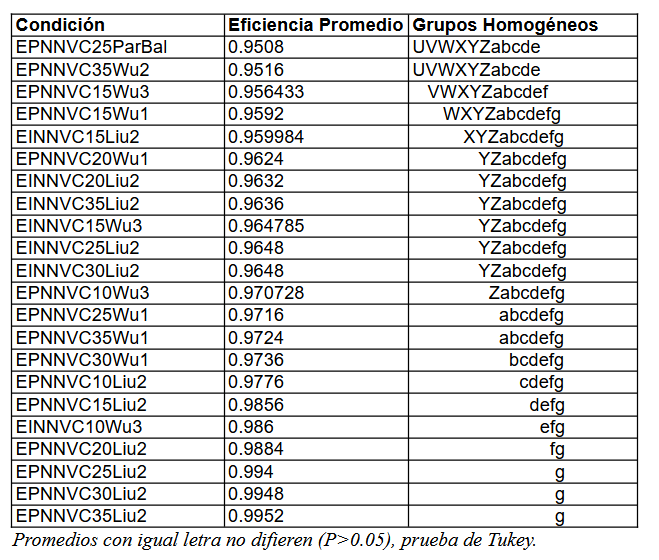
\includegraphics[width=0.76\linewidth]{img/CompEfic_PromICB_Perc_NNVC.png} 
	\caption{Comparación de eficiencias promedio del ICB Percentil cuando se tiene NNVC.} 
	\label{fig:CompEfic_PromICB_Perc_NNVC}
\end{figure}
\FloatBarrier



\subsubsection{Comparación de la eficiencia del ICB BCa cuando se tiene NNVC (NNVC-EficIB2)}

Cuando se tiene NNVC y se utilizó el ICB-BCa para evaluar la precisión, se obtuvo interacción triple significativa ($TipoMod*TM*Esq: F=5.95, P<0.0001$; Tabla \ref{fig:ANOVA_Efic_ICB_BCa_NNVC} del Anexo B). Con base en una eficiencia promedio de al menos 95\%, se obtuvo dos mejores esquemas Liu2 y Wu1 sin importar el TM, sin embargo, ambos sólo identifican al tipo de modelo EP a priori simulado (Tabla \ref{fig:CompEfic_PromICB_BCa_NNVC}). \\


\begin{figure}[ht] 
	\centering 
	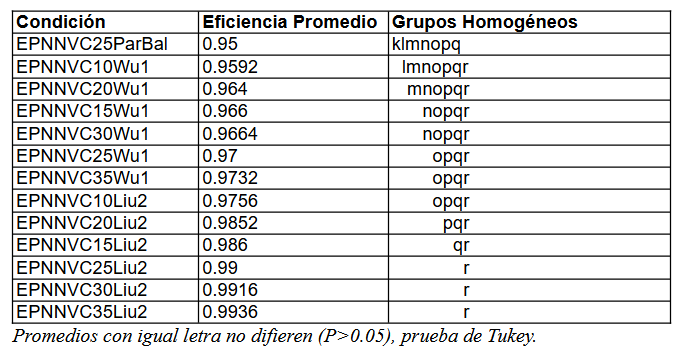
\includegraphics[width=0.76\linewidth]{img/CompEfic_PromICB_BCa_NNVC.png} 
	\caption{Comparación de eficiencias promedio del ICB BCa cuando se tiene NNVC.} 
	\label{fig:CompEfic_PromICB_BCa_NNVC}
\end{figure}
\FloatBarrier




%%%%%%%%%%%%%%%%%%%%%%%%%%%5
\subsubsection{Comparación de la eficiencia del ICB percentil cuando se tiene NVD (NVD-EficIB1)}

Cuando se tiene NVD y se utilizó el ICB-perc para evaluar la precisión, se obtuvo interacción triple significativa ($TipoMod*TM*Esq: F=7.89, P<0.0001;$ Tabla \ref{fig:ANOVA_Efic_ICB_Perc_NVD} del Anexo B). Con base en una eficiencia promedio de al menos 95\%, el mejor esquema resultó Liu2 sin importar el tamaño de muestra y tipo de modelo (Tabla \ref{fig:CompEfic_PromICB_Perc_NVD}).\\


\begin{figure}[ht] 
	\centering 
	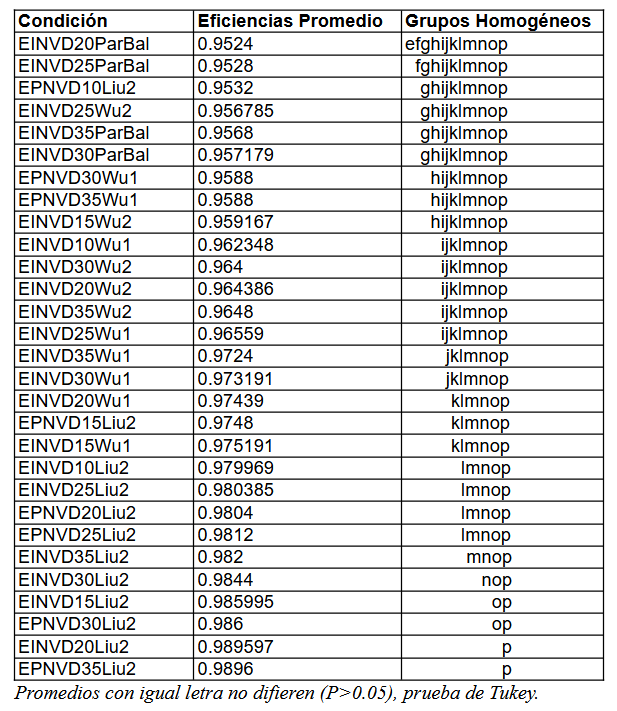
\includegraphics[width=0.76\linewidth]{img/CompEfic_PromICB_Perc_NVD.png} 
	\caption{Comparación de eficiencias promedio del ICB Percentil cuando se tiene NVD.} 
	\label{fig:CompEfic_PromICB_Perc_NVD}
\end{figure}
\FloatBarrier


\subsubsection{Comparación de la eficiencia del ICB BCa cuando se tiene NVD (NVD-EficIB2)}

Cuando se tiene NVD y se utilizó el ICB-BCa para evaluar la precisión, se obtuvo interacción triple significativa ($TipoMod*TM*Esq: F=3.91, P<0.0001;$ Tabla \ref{fig:ANOVA_Efic_ICB_BCa_NVD} del Anexo B). Con base en una eficiencia promedio de al menos 95\%, el mejor esquema resultó Liu2 sin importar el TM, sin embargo, sólo identifica al tipo de modelo EP a priori simulado (Tabla \ref{fig:CompEfic_PromICB_BCa_NVD})).\\

\begin{figure}[ht] 
	\centering 
	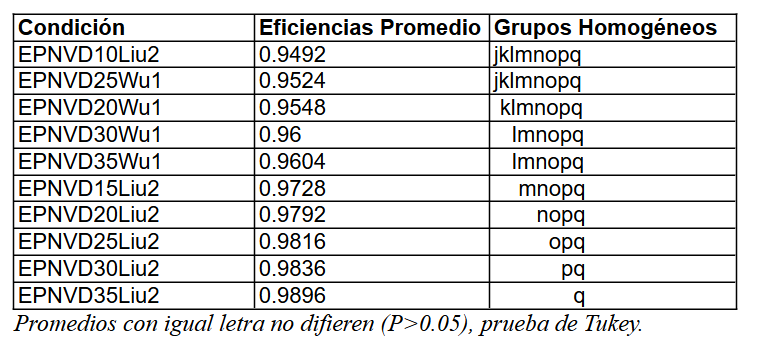
\includegraphics[width=0.76\linewidth]{img/CompEfic_PromICB_BCa_NVD.png} 
	\caption{Comparación de eficiencias promedio del ICB BCa cuando se tiene NVD.} 
	\label{fig:CompEfic_PromICB_BCa_NVD}
\end{figure}
\FloatBarrier



%%%%%%%%%%%%%%%%%%%%%%%%%%%5
\subsubsection{Comparación de la eficiencia del ICB percentil cuando se tiene NNVD (NNVD-EficIB1)}

Cuando se tiene NNVD y se utilizó el ICB-perc para evaluar la precisión, se obtuvo interacción triple significativa ($TipoMod*TM*Esq: F=10.71, P<0.0001;$ Tabla ~\ref{fig:ANOVA_Efic_ICB_Perc_NNVD} del Anexo B). Con base en una eficiencia promedio de al menos 93.96\%, se obtuvo dos mejores esquemas Liu2 y ParBal para todos los tamaños de muestra con excepción de n=35 para Liu2 (92.72\%) y n=10 para ParBal (91.28\%). Sin embargo, ambos esquemas sólo identifican al tipo de modelo EI a priori simulado (Tabla \ref{fig:CompEfic_PromICB_Perc_NNVD}).

\begin{figure}[ht] 
	\centering 
	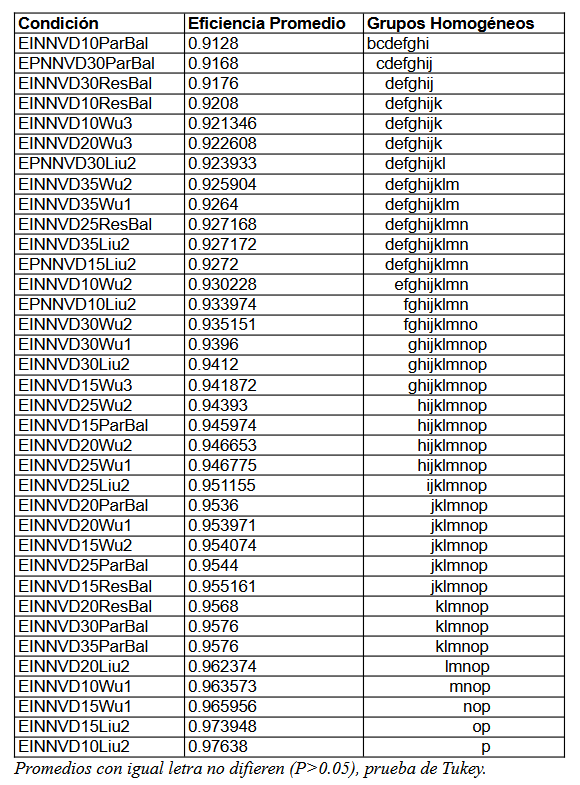
\includegraphics[width=0.76\linewidth]{img/CompEfic_PromICB_Perc_NNVD.png} 
	\caption{Comparación de eficiencias promedio del ICB Percentil cuando se tiene NVD.} 
	\label{fig:CompEfic_PromICB_Perc_NNVD}
\end{figure}
\FloatBarrier




\subsubsection{Comparación de la eficiencia del ICB BCa cuando se tiene NNVD (NNVD-EficIB2)}

Cuando se tiene NNVD y se utilizó el ICB-BCa para evaluar la precisión, se obtuvo interacción triple significativa ($TipoMod*TM*Esq: F=11.76, P<0.0001;$ Tabla \ref{fig:ANOVA_Efic_ICB_BCa_NNVD} del Anexo B). Con base en una eficiencia promedio de al menos 88.80\%, con el esquema ParBal se obtuvo la mayor eficiencia promedio en todos los tamaños de muestra, también bajo el esquema Liu2 con excepción de n=35 (88.80\%) cuando el tipo de modelo a priori simulado es EP. Cabe señalar que el esquema ParBal identifica el tipo de modelo EI para n=25, 30, 35 y las eficiencias no difieren estadísticamente con al menos 90.4\% (Tabla \ref{fig:CompEfic_PromICB_BCa_NNVD}).\\


\begin{figure}[ht] 
	\centering 
	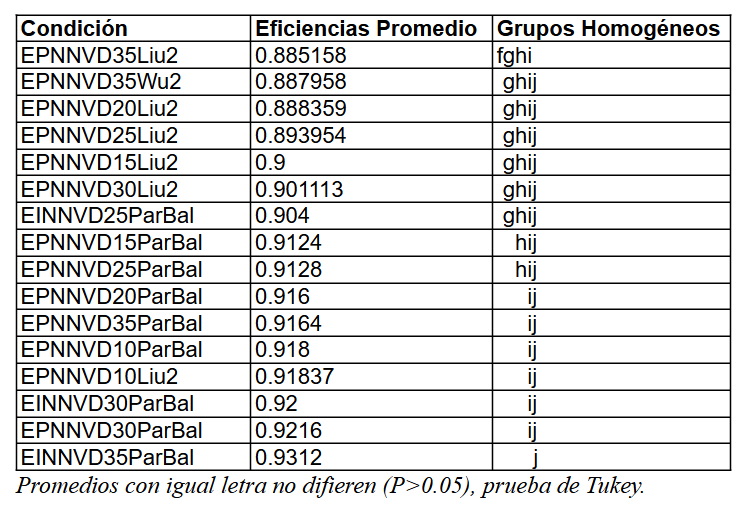
\includegraphics[width=0.76\linewidth]{img/CompEfic_PromICB_BCa_NNVD.png} 
	\caption{Comparación de eficiencias promedio del ICB BCa cuando se tiene NNVD.} 
	\label{fig:CompEfic_PromICB_BCa_NNVD}
\end{figure}
\FloatBarrier



\newpage

\subsection{Propuesta Final}

Con base en los resultados de los análisis estadísticos, cuando se tenga NVC, NNVC o NVD y se evalué la precisión el ICB a utilizar sería Percentil con esquema de remuestreo Liu2. Y cuando se tenga NNVD y se evalué la precisión, el ICB a utilizar sería BCa con esquema de remuestreo Pareado Balanceado.


\subsubsection{Implementación}


Para la propuesta final de este trabajo, dado los resultado estadísticos, para los diferentes casos NVC ,NNVC y NVD, se calcula el ICB Percentil para evaluar la precisión con el esquema de Liu2, ya que este obtuvo en el estudio de simulación una eficacia al menos del 95\%; con las diferencias en la implementación de los residuales: sea el caso 1 (NVC) utilizó los residuales al correr una regresión lineal simple, para el caso 2 (NVD) utilizó residuales robustos ponderados y el caso 3 (NNVC) los residuales robustos sin ponderar para la evaluación de precisión con un ICB. Ademas, cuando se tenga el caso 4 (NNVD) se evalúa la precisión con ICB BCa con el esquema de Remuestreo Balanceado que obtuvo una eficiencia al menos del 88.8\%.\\

La propuesta final se implemento en el lenguaje R, de tal forma que la evaluación de la precisión se realiza de manera automática dependiendo del
cumplimiento de los supuestos el resultados de las pruebas con una conclusión respectiva, los resultados estadísticos del ICB con el esquema Bootstrap y la conclusión si es un modelo preciso o impreciso dado: $\left( LI \leq 0.7 \leq LS \right) \; \text{o} \; \left( LI \geq 0.7 \right)$.\\

Solo es necesario proporcionar la muestra bivariada $(z_1, y_1), (z_2, y_2), \dots, (z_n, y_n)$ formada por los predichos $z_i$ y por los observados $y_i$ del modelo a evaluar y un nivel del confianza $1-\alpha$ para el ICB. Con un nivel de significancia $\alpha$ para el cumplimiento de los supuestos determinado por el nivel de confianza. La figura \ref{fig:propuestaFinal}  muestra el diagrama como funciona la propuesta final y en el Anexo C se encuentra el script R correspondiente a la función \textit{PropFCalcPrecModl()}.

\begin{figure}[ht!]
	\centering 
	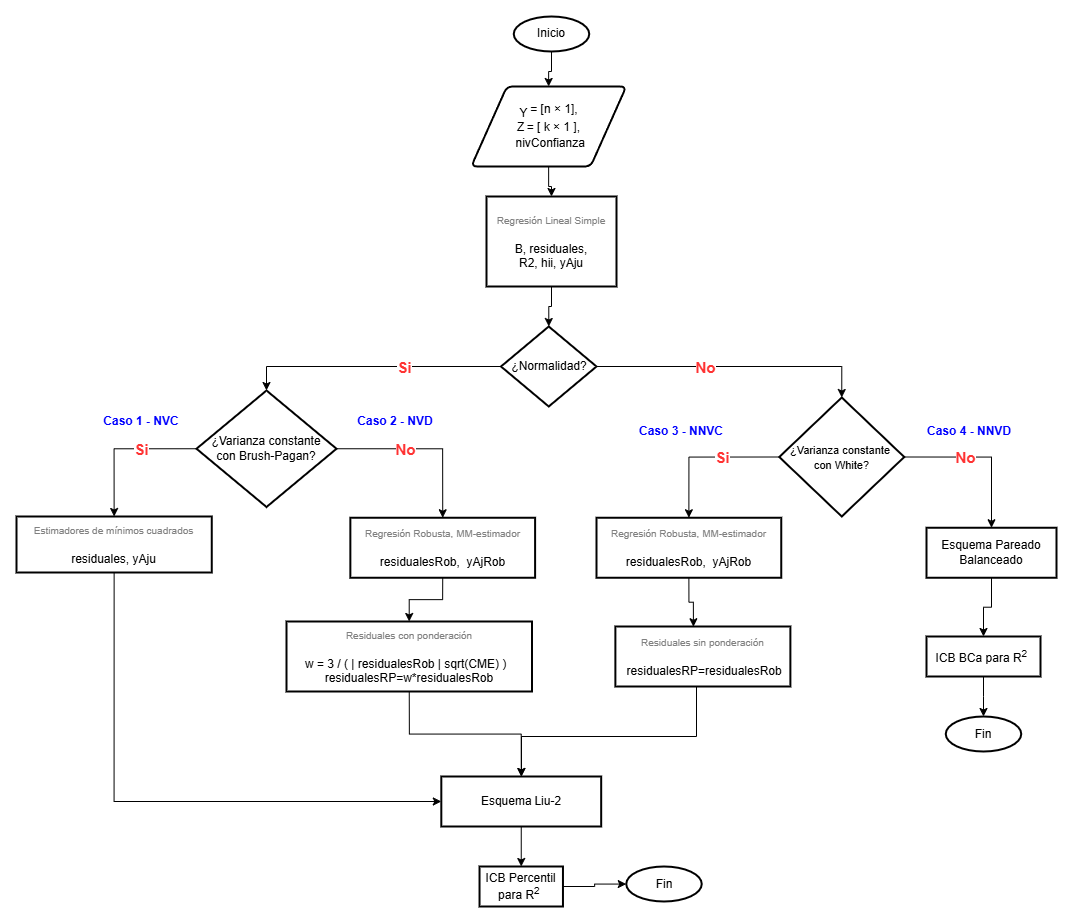
\includegraphics[width=0.9\linewidth]{img/propuestaFinalv7.png} 
	\caption{Propuesta final para evaluar la precisión de un modelo.}
	\label{fig:propuestaFinal}
\end{figure}
\FloatBarrier

\subsubsection{Aplicación}



\textbf{Caso 1 - NVC}

Para este caso se consideraron los datos experimentales de la ganancia diaria de peso (GDP); datos experimentales vs. modelo de simulación para estimar la ganancia diaria de peso (GDP) \parencite{osorio-2011}. Estos datos se encuentran en el apéndice B de \textcite{balam-2012}.\\


Con base en los resultados de verificación de los supuestos (Figura \ref{fig:final_NVC_resultados}) se obtuvo que corresponde al caso NVC. Por lo tanto para la evaluación de la precisión se aplicó el ICB Percentil con el esquema de remuestreo Liu2, dando como resultado que el modelo evaluado es preciso considerando un $R^2 \geq 70\%$.


\begin{figure}[ht!]
	\centering 
	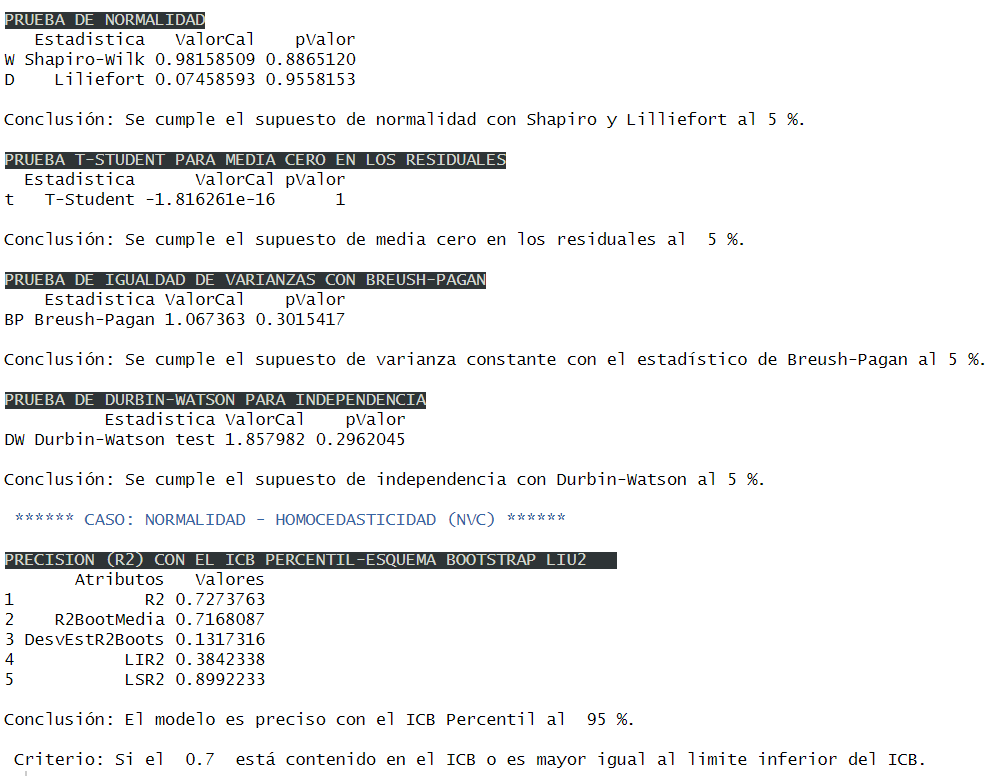
\includegraphics[width=0.85\linewidth]{img/Uso_NVC_PropuestaFinal.png} 
	\caption{Resultados del caso NVC.}
	\label{fig:final_NVC_resultados}
\end{figure}
\FloatBarrier







\textbf{Caso 2 - NNVD}\\

Se aplico a los datos experimentales del volumen de una parcela en metros cúbicos a un diámetro superior $(n = 63)$ de 10cm y los simulados con el modelo PTAEDA \parencite{chung-1987}, el cual es un modelo estocástico. Cada simulación 86 con el modelo PTAEDA corresponde a la media de 10 corridas del modelo para cada parcela. En cada parcela se mide la edad, el indice de sitio y el número de arboles por hectárea.Estos datos se encuentran en el apéndice B de \textcite{balam-2012}.\\


Con base en los resultados de verificación de los supuestos (Figura \ref{fig:final_NNVD_resultados}) se obtuvo que corresponde al caso NNVD. Por lo tanto para la evaluación de la precisión se aplicó el ICB BCa con el esquema de remuestreo Pareado Balanceado, dando como resultado que el modelo evaluado es preciso considerando un $R^2 \geq 70\%$.

\begin{figure}[ht!]
	\centering 
	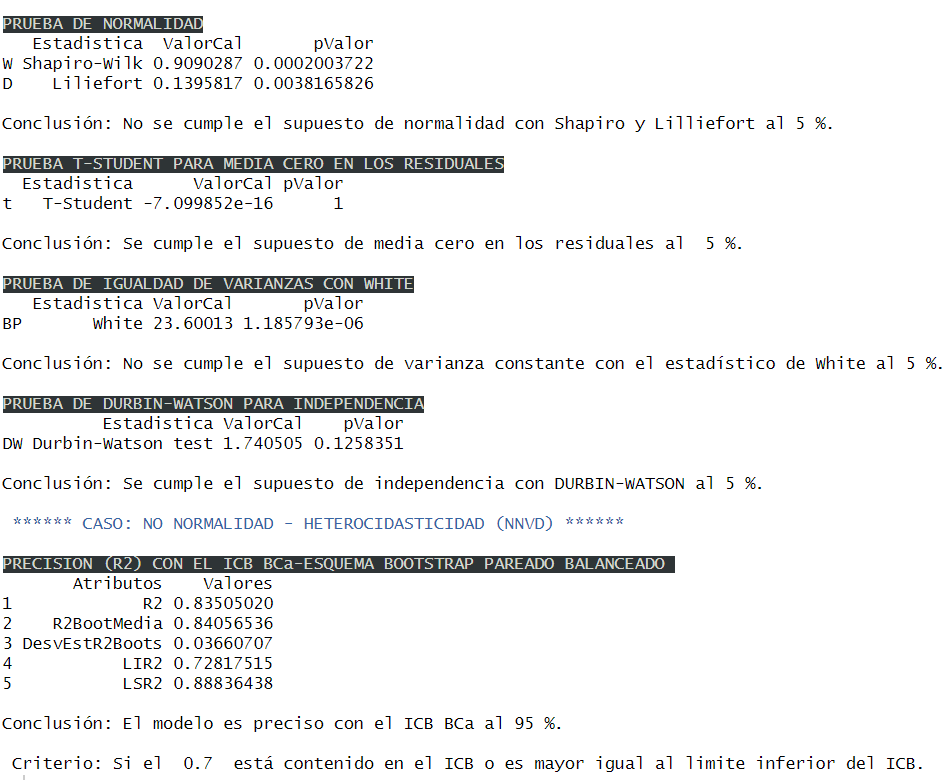
\includegraphics[width=0.85\linewidth]{img/Uso_NNVD_PropuestaFinal.png} 
	\caption{Resultados del caso NNVD.}
	\label{fig:final_NNVD_resultados}
\end{figure}
\FloatBarrier




